% Workstream structural: supplementary tables and figures, generated by
% `python -m albert.research.flb_structural run latex` and paper_flb/scripts/fig_structural.py from
% data/research/flb_structural/ (band_cells.csv, band_tick_grid.csv, weighting_*.csv, shin_*.csv,
% beliefs_coef.csv, decomposition.csv, summary.json).

This appendix supports \cref{sec:res-structural}. The CSV files under \texttt{data/research/flb\_structural/} also
hold every bucket $\times$ lead $\times$ group cell of the band, the fits for each group and lead, and the $\shinz$ of
every event-lead.
\begin{itemize}
  \item \emph{Band.} \Cref{tab:structural-band-groups} splits the band decomposition by price bucket and group.
  \Cref{tab:structural-band-robust} varies:
  \begin{itemize}
    \item the cost of capital;
    \item the weights;
    \item the sample half;
    \item the quote age and the spread;
    \item the tick grid and the contract structure.
  \end{itemize}
  It also drops the five events with the largest absolute contribution to the residual.
  \item \emph{Weighting.} \Cref{tab:structural-weighting-cells,fig:structural-weighting} give the weighting
  functions by lead, structure and group.
  \item \emph{Shin.} \Cref{tab:structural-shin-full,tab:structural-shin-forecasts,fig:structural-shin} give
  $\shinz$ by lead, group and structure, and compare forecasts.
  \item \emph{Belief dispersion.} \Cref{tab:structural-beliefs,tab:structural-beliefs-groups,fig:structural-beliefs}
  report the slope interactions, pooled, by group and by half.
  \item \emph{Synthesis.} \Cref{tab:structural-scorecard} lists every prediction tested and
  \cref{tab:structural-decomp} the counterfactual shares.
\end{itemize}

% BEGIN AUTO:tab-band-groups
\begin{table}[!htbp]
\centering
\begin{threeparttable}
\caption{The band by group and longshot bucket}\label{tab:structural-band-groups}
\scriptsize
\setlength{\tabcolsep}{3pt}
\begin{tabular}{@{}lrrrrrrrrrrr@{}}
\toprule
 & & & & Gross & \multicolumn{4}{c}{Band components} & Residual & Maker & In band \\
\cmidrule(lr){6-9}
Cell & Sides & Events & $\bar\q$ & $\bar\q-\bar\won$ & Floor & Half-spr. & Fee & Capital & $\bar R$ & $\bar R^{mk}$ & (\%) \\
\midrule
% source: data/research/flb_structural/band_cells.csv
\multicolumn{12}{@{}l}{\emph{All groups}} \\
\quad 1--2\cents & 26{,}184 & 2{,}118 & 0.87 & 0.49 (6.9) & 0.30 & 0.48 & 0.01 & 0.03 & $-$0.33 ($-$4.6) & 1.24 (16.9) & 100 \\
\quad 3--5\cents & 9{,}521 & 2{,}007 & 3.53 & 1.86 (9.0) & 0.00 & 2.40 & 0.08 & 0.04 & $-$0.65 ($-$3.2) & 4.21 (19.4) & 100 \\
\quad 6--10\cents & 4{,}847 & 1{,}707 & 7.53 & 2.01 (4.1) & 0.00 & 2.22 & 0.34 & 0.04 & $-$0.60 ($-$1.2) & 4.18 (8.4) & 100 \\
\multicolumn{12}{@{}l}{\emph{Sports}} \\
\quad 1--2\cents & 6{,}211 & 303 & 0.79 & 0.46 (3.1) & 0.35 & 0.39 & 0.00 & 0.05 & $-$0.32 ($-$2.2) & 1.14 (7.4) & 100 \\
\quad 3--5\cents & 1{,}914 & 280 & 3.56 & 2.25 (5.8) & 0.00 & 2.67 & 0.06 & 0.04 & $-$0.52 ($-$1.4) & 4.85 (11.3) & 100 \\
\quad 6--10\cents & 983 & 276 & 7.63 & 2.02 (1.7) & 0.00 & 2.21 & 0.32 & 0.03 & $-$0.54 ($-$0.5) & 4.16 (3.4) & 100 \\
\multicolumn{12}{@{}l}{\emph{Weather}} \\
\quad 1--2\cents & 2{,}126 & 317 & 0.97 & 0.24 (0.7) & 0.27 & 0.56 & 0.01 & 0.03 & $-$0.63 ($-$1.9) & 1.04 (3.2) & 100 \\
\quad 3--5\cents & 1{,}122 & 455 & 3.68 & 1.57 (2.6) & 0.00 & 2.38 & 0.09 & 0.02 & $-$0.92 ($-$1.5) & 3.94 (6.4) & 100 \\
\quad 6--10\cents & 657 & 384 & 7.52 & 3.29 (3.4) & 0.00 & 2.33 & 0.34 & 0.02 & 0.59 (0.6) & 5.60 (5.8) & 82 \\
\multicolumn{12}{@{}l}{\emph{Politics}} \\
\quad 1--2\cents & 7{,}720 & 728 & 0.93 & 0.41 (2.7) & 0.25 & 0.56 & 0.01 & 0.03 & $-$0.44 ($-$2.9) & 1.19 (7.9) & 100 \\
\quad 3--5\cents & 2{,}597 & 563 & 3.49 & 0.66 (1.2) & 0.00 & 2.14 & 0.09 & 0.05 & $-$1.62 ($-$3.0) & 2.76 (5.1) & 100 \\
\quad 6--10\cents & 1{,}451 & 482 & 7.54 & 0.70 (0.7) & 0.00 & 2.17 & 0.35 & 0.06 & $-$1.89 ($-$1.9) & 2.81 (2.8) & 100 \\
\multicolumn{12}{@{}l}{\emph{Entertainment}} \\
\quad 1--2\cents & 6{,}011 & 377 & 0.90 & 0.66 (6.1) & 0.29 & 0.54 & 0.00 & 0.02 & $-$0.20 ($-$1.9) & 1.47 (12.3) & 100 \\
\quad 3--5\cents & 2{,}169 & 353 & 3.48 & 2.77 (10.2) & 0.00 & 2.76 & 0.05 & 0.04 & $-$0.09 ($-$0.3) & 5.49 (18.6) & 100 \\
\quad 6--10\cents & 759 & 266 & 7.39 & 1.74 (1.3) & 0.00 & 2.33 & 0.33 & 0.07 & $-$0.99 ($-$0.7) & 4.01 (2.9) & 100 \\
\multicolumn{12}{@{}l}{\emph{Mentions}} \\
\quad 1--2\cents & 982 & 58 & 0.72 & 0.72 (24.0) & 0.39 & 0.18 & 0.01 & 0.02 & 0.12 (5.9) & 1.27 (25.0) & 83 \\
\quad 3--5\cents & 423 & 64 & 3.60 & 2.57 (5.7) & 0.00 & 1.53 & 0.14 & 0.02 & 0.88 (2.0) & 4.08 (7.5) & 66 \\
\quad 6--10\cents & 513 & 82 & 7.65 & 2.38 (1.6) & 0.00 & 2.02 & 0.37 & 0.02 & $-$0.03 (0.0) & 4.38 (2.9) & 100 \\
\multicolumn{12}{@{}l}{\emph{Science \& Tech}} \\
\quad 1--2\cents & 2{,}967 & 311 & 0.87 & 0.48 (2.4) & 0.30 & 0.47 & 0.01 & 0.03 & $-$0.33 ($-$1.6) & 1.21 (5.8) & 100 \\
\quad 3--5\cents & 1{,}184 & 267 & 3.38 & 1.93 (3.2) & 0.00 & 2.13 & 0.09 & 0.06 & $-$0.35 ($-$0.6) & 3.97 (6.4) & 100 \\
\quad 6--10\cents & 421 & 189 & 7.37 & 2.48 (1.7) & 0.00 & 2.24 & 0.34 & 0.09 & $-$0.19 ($-$0.1) & 4.60 (3.1) & 100 \\
\bottomrule
\end{tabular}
\begin{tablenotes}\footnotesize
\item As \cref{tab:structural-band}, by group and price bucket, leads pooled, $\rho=5\%$, market-weighted. $t$-statistics clustered by event in parentheses.
\end{tablenotes}
\end{threeparttable}
\end{table}
% END AUTO:tab-band-groups

% BEGIN AUTO:tab-band-robust
\begin{table}[!htbp]
\centering
\begin{threeparttable}
\caption{The band: cost of capital, weights, halves and the tick grid}\label{tab:structural-band-robust}
\scriptsize
\setlength{\tabcolsep}{2.5pt}
\begin{tabular}{@{}lrrrrrrrrrrr@{}}
\toprule
 & & & & Gross & \multicolumn{4}{c}{Band components} & Residual & Maker & In band \\
\cmidrule(lr){6-9}
Cell & Sides & Events & $\bar\q$ & $\bar\q-\bar\won$ & Floor & Half-spr. & Fee & Capital & $\bar R$ & $\bar R^{mk}$ & (\%) \\
\midrule
% source: data/research/flb_structural/band_cells.csv, summary.json:band.robustness, band_tick_grid.csv
Main & 40{,}552 & 3{,}091 & 2.54 & 1.07 (10.0) & 0.18 & 1.23 & 0.07 & 0.04 & $-$0.45 ($-$4.3) & 2.44 (21.3) & 100 \\
$\rho=0$ & 40{,}552 & 3{,}091 & 2.54 & 1.07 (10.0) & 0.18 & 1.23 & 0.07 & 0.00 & $-$0.42 ($-$3.9) & 2.47 (21.6) & 100 \\
$\rho=10\%$ & 40{,}552 & 3{,}091 & 2.54 & 1.07 (10.0) & 0.18 & 1.23 & 0.07 & 0.07 & $-$0.49 ($-$4.6) & 2.40 (20.9) & 100 \\
Volume-weighted & 40{,}552 & 3{,}091 & 2.18 & 1.56 (5.1) & 0.27 & 0.39 & 0.10 & 0.02 & 0.79 (2.7) & 2.19 (7.3) & 50 \\
First half (to 2025-07) & 22{,}146 & 1{,}762 & 2.67 & 0.81 (5.1) & 0.17 & 1.30 & 0.08 & 0.03 & $-$0.76 ($-$4.8) & 2.24 (13.3) & 100 \\
Second half & 18{,}406 & 1{,}341 & 2.69 & 0.97 (5.4) & 0.18 & 1.19 & 0.08 & 0.04 & $-$0.52 ($-$2.9) & 2.29 (12.2) & 100 \\
Drop 5 influential events & 40{,}507 & 3{,}086 & 2.54 & 1.16 (11.7) & 0.18 & 1.23 & 0.07 & 0.04 & $-$0.36 ($-$3.7) & 2.53 (23.6) & 100 \\
Quote age $\le$ 24 h & 33{,}432 & 3{,}055 & 2.72 & 1.11 (9.2) & 0.16 & 1.29 & 0.08 & 0.04 & $-$0.46 ($-$3.9) & 2.52 (19.7) & 100 \\
Spread $\le$ 5\cents & 35{,}751 & 2{,}868 & 2.11 & 0.80 (7.4) & 0.21 & 0.80 & 0.07 & 0.04 & $-$0.31 ($-$2.9) & 1.77 (16.0) & 100 \\
Pinned at the floor & 15{,}801 & 1{,}445 & 0.50 & 0.37 (7.5) & 0.50 & 0.00 & 0.00 & 0.03 & $-$0.16 ($-$3.3) & 0.83 (16.9) & 100 \\
Above the floor & 24{,}751 & 2{,}889 & 3.67 & 1.46 (9.1) & 0.00 & 1.91 & 0.11 & 0.04 & $-$0.61 ($-$3.8) & 3.33 (20.1) & 100 \\
With a bid ($\q^b>0$) & 12{,}404 & 2{,}494 & 4.98 & 1.42 (5.3) & 0.00 & 1.68 & 0.22 & 0.04 & $-$0.52 ($-$1.9) & 3.05 (11.3) & 100 \\
Binary & 8{,}484 & 1{,}324 & 3.26 & 1.58 (6.5) & 0.12 & 1.47 & 0.11 & 0.03 & $-$0.14 ($-$0.6) & 3.14 (12.4) & 100 \\
Multi-outcome & 10{,}045 & 291 & 1.69 & 1.04 (7.3) & 0.27 & 0.89 & 0.03 & 0.04 & $-$0.20 ($-$1.5) & 2.16 (12.1) & 100 \\
Ladder leg & 13{,}819 & 884 & 2.87 & 0.84 (3.9) & 0.13 & 1.42 & 0.09 & 0.03 & $-$0.83 ($-$3.9) & 2.35 (10.6) & 100 \\
Deadline & 8{,}204 & 608 & 2.10 & 0.90 (4.1) & 0.22 & 1.01 & 0.06 & 0.07 & $-$0.46 ($-$2.1) & 2.06 (8.9) & 100 \\
1\cents{} grid, 1--2\cents & 25{,}800 & 2{,}093 & 0.87 & 0.49 (6.8) & 0.30 & 0.48 & 0.01 & 0.03 & $-$0.34 ($-$4.7) & 1.24 (16.7) & 100 \\
0.1\cents{} grid, 1--2\cents & 384 & 31 & 0.75 & 0.75 (10.2) & 0.01 & 0.50 & 0.02 & 0.05 & 0.17 (2.3) & 1.20 (8.7) & 77 \\
1\cents{} grid, all \LS & 39{,}960 & 3{,}061 & 2.55 & 1.07 (9.9) & 0.18 & 1.23 & 0.07 & 0.04 & $-$0.45 ($-$4.3) & 2.44 (21.2) & 100 \\
0.1\cents{} grid, all \LS & 592 & 36 & 1.94 & 0.92 (1.3) & 0.00 & 1.01 & 0.06 & 0.07 & $-$0.24 ($-$0.3) & 1.87 (2.5) & 100 \\
\bottomrule
\end{tabular}
\begin{tablenotes}\footnotesize
\item Longshot sides ($\q\le10\cents$ at the mid), leads pooled; columns as in \cref{tab:structural-band}. Halves split at the month that divides the quotes most evenly. The influential events are the five with the largest absolute contribution to the residual. Grid: markets quoted on Kalshi's 0.1\cents{} price grid against the standard 1\cents{} grid; the floor is one tick on each grid. $t$-statistics clustered by event in parentheses.
\end{tablenotes}
\end{threeparttable}
\end{table}
% END AUTO:tab-band-robust

\begin{figure}[!htbp]
\centering
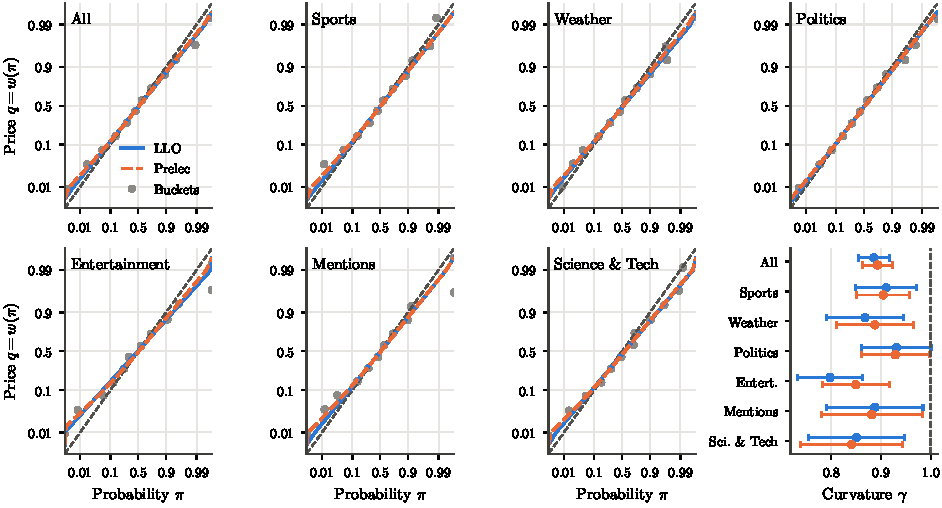
\includegraphics[width=\textwidth]{figures/fig_structural_weighting.pdf}
\caption{Fitted probability-weighting functions $\q=w(\pi)$ on log-odds axes: linear in log odds (LLO) and Prelec,
pooled and by group, with the calibration points (realised frequency, mean YES price) of the price buckets.
Buckets with no or only winning outcomes sit at the edges. The dashed diagonal is calibration. Last panel:
curvature $\gamma$ by group with 95\% confidence intervals clustered by event (LLO upper, Prelec lower marker).
YES sides of pre-event quotes, market-weighted.}\label{fig:structural-weighting}
\end{figure}

% BEGIN AUTO:tab-weighting-cells
\begin{table}[!htbp]
\centering
\begin{threeparttable}
\caption{Weighting-function parameters by lead and structure}\label{tab:structural-weighting-cells}
\scriptsize
\setlength{\tabcolsep}{3pt}
\begin{tabular}{@{}lrrrrrrrr@{}}
\toprule
 & & & \multicolumn{4}{c}{LLO} & \multicolumn{2}{c}{Prelec} \\
\cmidrule(lr){4-7}\cmidrule(l){8-9}
Cell & Quotes & Events & $\alpha$ & $\beta$ ($t_{\beta=1}$) & $\gamma$ & $\delta$ & $\gamma$ & $\delta$ \\
\midrule
% source: data/research/flb_structural/weighting_fits.csv
\multicolumn{9}{@{}l}{\emph{By lead}} \\
\quad 1h & 15{,}784 & 4{,}191 & 0.06 & 1.18 (7.1) & 0.85 (0.018) & $-$0.05 (0.033) & 0.87 (0.018) & 1.00 (0.018) \\
\quad 6h & 15{,}827 & 4{,}163 & 0.07 & 1.20 (7.7) & 0.84 (0.018) & $-$0.06 (0.032) & 0.85 (0.017) & 1.00 (0.017) \\
\quad 24h & 11{,}688 & 2{,}739 & 0.13 & 1.23 (7.8) & 0.81 (0.020) & $-$0.11 (0.040) & 0.83 (0.020) & 1.03 (0.022) \\
\quad 3d & 10{,}358 & 2{,}380 & 0.03 & 1.17 (5.9) & 0.86 (0.021) & $-$0.02 (0.045) & 0.89 (0.022) & 0.99 (0.024) \\
\quad 7d & 5{,}553 & 1{,}478 & $-$0.12 & 1.16 (3.8) & 0.86 (0.031) & 0.10 (0.069) & 0.91 (0.033) & 0.92 (0.036) \\
\quad 30d & 2{,}782 & 885 & $-$0.32 & 1.12 (2.3) & 0.89 (0.043) & 0.28 (0.087) & 0.98 (0.048) & 0.83 (0.041) \\
\multicolumn{9}{@{}l}{\emph{By structure}} \\
\quad Binary & 17{,}163 & 2{,}644 & $-$0.04 & 1.12 (3.7) & 0.89 (0.026) & 0.04 (0.038) & 0.91 (0.023) & 0.96 (0.022) \\
\quad Multi-outcome & 12{,}822 & 474 & 0.14 & 1.28 (4.4) & 0.78 (0.039) & $-$0.11 (0.037) & 0.84 (0.032) & 1.01 (0.013) \\
\quad Ladder leg & 22{,}392 & 1{,}030 & 0.14 & 1.12 (2.9) & 0.89 (0.032) & $-$0.13 (0.062) & 0.89 (0.033) & 1.05 (0.033) \\
\quad Deadline & 9{,}615 & 644 & 0.47 & 1.22 (3.9) & 0.82 (0.039) & $-$0.38 (0.108) & 0.77 (0.041) & 1.21 (0.067) \\
\multicolumn{9}{@{}l}{\emph{By group, volume-weighted}} \\
\quad All groups & 46{,}505 & 4{,}430 & $-$0.01 & 1.48 (3.6) & 0.68 (0.061) & 0.01 (0.130) & 0.76 (0.064) & 0.96 (0.082) \\
\quad Sports & 11{,}242 & 1{,}298 & $-$0.29 & 1.37 (2.0) & 0.73 (0.098) & 0.21 (0.119) & 0.86 (0.089) & 0.83 (0.067) \\
\quad Weather & 5{,}616 & 1{,}007 & $-$0.10 & 1.29 (2.0) & 0.77 (0.089) & 0.07 (0.133) & 0.86 (0.079) & 0.92 (0.068) \\
\quad Politics & 12{,}490 & 941 & 1.13 & 1.80 (6.6) & 0.56 (0.038) & $-$0.63 (0.305) & 0.53 (0.063) & 1.39 (0.228) \\
\quad Entertainment & 7{,}609 & 506 & 0.76 & 1.34 (3.0) & 0.74 (0.064) & $-$0.57 (0.249) & 0.68 (0.060) & 1.34 (0.164) \\
\quad Mentions & 4{,}517 & 102 & 0.07 & 1.35 (4.6) & 0.74 (0.041) & $-$0.05 (0.116) & 0.77 (0.044) & 0.99 (0.064) \\
\quad Science \& Tech & 4{,}678 & 503 & $-$0.13 & 1.56 (4.0) & 0.64 (0.058) & 0.08 (0.170) & 0.73 (0.058) & 0.92 (0.092) \\
\quad Other & 353 & 73 & 0.34 & 1.43 (1.5) & 0.70 (0.144) & $-$0.24 (0.361) & 0.71 (0.134) & 1.11 (0.230) \\
\bottomrule
\end{tabular}
\begin{tablenotes}\footnotesize
\item As \cref{tab:structural-weighting}. Within a lead each market counts once. Standard errors (or $t$) clustered by event in parentheses.
\end{tablenotes}
\end{threeparttable}
\end{table}
% END AUTO:tab-weighting-cells

\begin{figure}[!htbp]
\centering
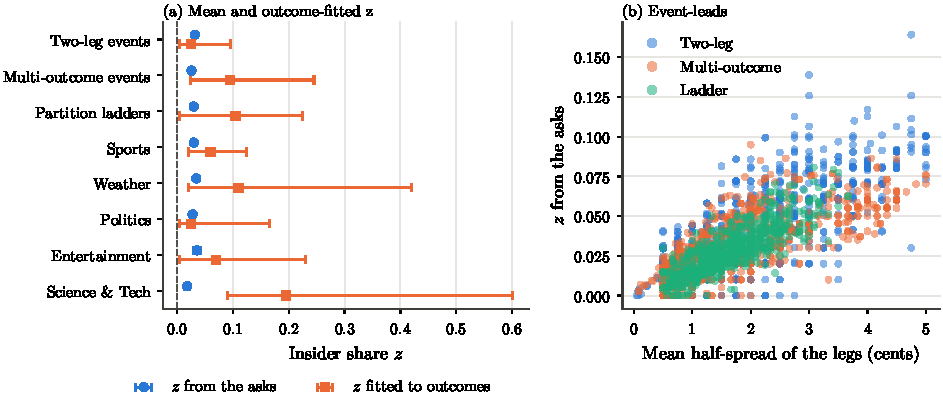
\includegraphics[width=\textwidth]{figures/fig_structural_shin.pdf}
\caption{Shin's insider share in partition events. Left: mean $\shinz$ implied by the asks (95\% confidence
intervals clustered by event) and $\shinz$ fitted to outcomes (95\% event-bootstrap intervals; the grid ends at
0.6), by structure and group. Right: $\shinz$ implied by the asks against the mean half-spread of the event's
legs, one point per event and lead.}\label{fig:structural-shin}
\end{figure}

% BEGIN AUTO:tab-shin-full
\begin{table}[!htbp]
\centering
\begin{threeparttable}
\caption{Shin's insider share by lead, group and structure}\label{tab:structural-shin-full}
\scriptsize
\setlength{\tabcolsep}{2.8pt}
\begin{tabular}{@{}lrrrrrrrr@{}}
\toprule
 & Event- & & Legs & $\sum a-1$ & $\sum p-1$ & $\shinz$ from & $\shinz$ from & $\shinz$ fitted \\
Sample & leads & Events & (med.) & (\%) & (\%) & asks & mids & to outcomes [95\% CI] \\
\midrule
% source: data/research/flb_structural/shin_cells.csv
\multicolumn{9}{@{}l}{\emph{By lead}} \\
\quad 1h & 1{,}143 & 1{,}143 & 2 & 6.9 (24.9) & 1.2 (9.1) & 0.031 (0.0008) & 0.004 & 0.060 [0.025, 0.135] \\
\quad 6h & 1{,}187 & 1{,}187 & 2 & 7.4 (23.2) & 1.2 (7.5) & 0.030 (0.0007) & 0.005 & 0.135 [0.075, 0.225] \\
\quad 24h & 729 & 729 & 3 & 8.4 (20.7) & 1.4 (8.2) & 0.030 (0.0008) & 0.004 & 0.115 [0.065, 0.185] \\
\quad 3d & 559 & 559 & 3 & 10.6 (18.3) & 1.9 (8.8) & 0.027 (0.0009) & 0.004 & 0.010 [0.000, 0.095] \\
\quad 7d & 242 & 242 & 2 & 8.1 (9.4) & 1.6 (3.9) & 0.030 (0.0013) & 0.005 & 0.010 [0.000, 0.080] \\
\quad 30d & 95 & 95 & 2 & 10.1 (6.9) & 1.8 (2.5) & 0.038 (0.0032) & 0.007 & 0.020 [0.000, 0.600] \\
\multicolumn{9}{@{}l}{\emph{By group and structure}} \\
\quad Sports, two-leg & 1{,}609 & 660 & 2 & 3.1 (38.3) & $-$0.2 ($-$4.2) & 0.032 (0.0008) & 0.003 & 0.020 [0.000, 0.095] \\
\quad Sports, multi & 764 & 256 & 3 & 9.0 (12.4) & 1.4 (4.1) & 0.026 (0.0010) & 0.003 & 0.155 [0.035, 0.530] \\
\quad Weather, partition ladder & 237 & 139 & 6 & 15.5 (25.5) & 4.1 (11.4) & 0.034 (0.0014) & 0.010 & 0.110 [0.020, 0.420] \\
\quad Politics, two-leg & 376 & 74 & 2 & 2.5 (13.9) & 0.0 (0.0) & 0.031 (0.0020) & 0.003 & 0.050 [0.015, 0.370] \\
\quad Politics, multi & 217 & 46 & 6 & 11.5 (11.8) & 3.2 (7.5) & 0.030 (0.0024) & 0.008 & 0.020 [0.005, 0.331] \\
\quad Politics, partition ladder & 418 & 160 & 9 & 17.7 (29.4) & 3.7 (11.8) & 0.026 (0.0009) & 0.006 & 0.100 [0.000, 0.265] \\
\quad Entertainment, two-leg & 24 & 6 & 2 & 4.3 (4.8) & 0.5 (2.0) & 0.057 (0.0132) & 0.006 & 0.600 [0.600, 0.600] \\
\quad Entertainment, multi & 94 & 35 & 10 & 19.6 (8.4) & 6.9 (6.0) & 0.032 (0.0031) & 0.010 & 0.035 [0.000, 0.220] \\
\quad Science \& Tech, multi & 214 & 44 & 7 & 7.6 (5.4) & 1.8 (2.3) & 0.018 (0.0019) & 0.005 & 0.195 [0.090, 0.600] \\
\bottomrule
\end{tabular}
\begin{tablenotes}\footnotesize
\item As \cref{tab:structural-shin}. Regression of $\shinz$ from the asks on the mean half-spread, log legs and group dummies (Sports omitted), weighted, event-clustered $t$ in parentheses: half-spread (\cents) 0.0168 (50.5); log legs $-$0.0037 ($-$5.8); Weather 0.0029 (2.7); Politics 0.0039 (4.7); Entertainment 0.0114 (5.7); Science \& Tech 0.0059 (4.2); $R^2=0.68$, 3{,}955 event-leads.
\end{tablenotes}
\end{threeparttable}
\end{table}
% END AUTO:tab-shin-full

% BEGIN AUTO:tab-shin-forecasts
\begin{table}[!htbp]
\centering
\begin{threeparttable}
\caption{Partition events: raw, normalised and Shin probabilities}\label{tab:structural-shin-forecasts}
\footnotesize
\setlength{\tabcolsep}{3.5pt}
\begin{tabular}{@{}lrrrrl@{}}
\toprule
 & \multicolumn{2}{c}{Longshot legs (\cents)} & \multicolumn{3}{c}{Log score gain (milli-nats)} \\
\cmidrule(lr){2-3}\cmidrule(l){4-6}
Forecast & All months & Second half & All months & Second half & against \\
\midrule
% source: data/research/flb_structural/summary.json:shin.longshot_legs, shin_scores.csv
Raw mid & 0.93 (4.9) & 1.08 (4.3) & -- & -- & -- \\
Normalised mids & 0.83 (4.4) & 1.01 (4.1) & $-$0.41 ($-$3.2) & $-$0.69 ($-$3.6) & raw mid \\
Normalised asks & -- & -- & -- & -- & -- \\
Shin, from the asks & 0.94 (5.0) & 1.06 (4.3) & 3.47 (8.5) & 3.47 (6.2) & normalised asks \\
Shin, from the mids & -- & -- & 0.86 (5.0) & 0.89 (3.3) & normalised mids \\
Shin, $\shinz$ fitted on the first half & $-$0.21 ($-$1.1) & 0.05 (0.2) & 1.45 (1.7) & 1.79 (1.5) & normalised mids \\
\bottomrule
\end{tabular}
\begin{tablenotes}\footnotesize
\item Legs of the partition events of \cref{tab:structural-shin}. Longshot legs: mid at most 10\cents{} (8{,}906 legs in all months, 3{,}747 in the second half); mean forecast minus outcome in cents. Log score: mean gain per leg, over all legs, against the normalisation of the same prices. The fitted $\shinz$ is estimated on the first half of the months, so the second half is out of sample. Each event weighs one across its leads; $t$-statistics clustered by event in parentheses.
\end{tablenotes}
\end{threeparttable}
\end{table}
% END AUTO:tab-shin-forecasts

\begin{figure}[!htbp]
\centering
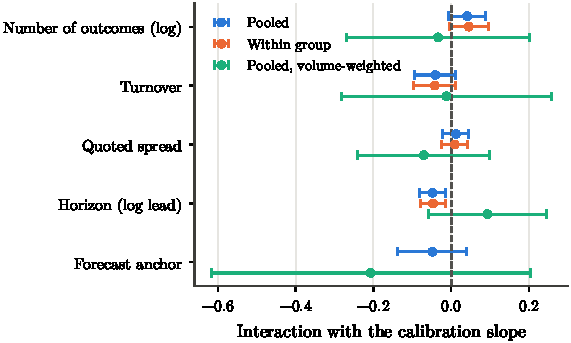
\includegraphics[width=0.66\textwidth]{figures/fig_structural_beliefs.pdf}
\caption{Interaction of each characteristic with the calibration slope, $b_k$ in~\eqref{eq:structural-interact}:
the change in the logit slope per standard deviation (per unit for the 0/1 anchor). Positive values mean a stronger
favourite--longshot bias. Pooled, within groups (group-specific slopes; the anchor is absorbed) and pooled
volume-weighted. 95\% confidence intervals clustered by event.}\label{fig:structural-beliefs}
\end{figure}

% BEGIN AUTO:tab-beliefs
\begin{table}[!htbp]
\centering
\begin{threeparttable}
\caption{Where is the bias steeper? Calibration-slope interactions}\label{tab:structural-beliefs}
\scriptsize
\setlength{\tabcolsep}{3.5pt}
\begin{tabular}{@{}lrrrrrr@{}}
\toprule
 & \multicolumn{4}{c}{Slope interaction (logit)} & \multicolumn{2}{c}{Longshot overpricing (\cents)} \\
\cmidrule(lr){2-5}\cmidrule(l){6-7}
 & Pooled & Within group & Volume-wtd. & Split anchor & Within group & Split anchor \\
\midrule
% source: data/research/flb_structural/beliefs_coef.csv
Number of outcomes (log) & 0.041 (1.7) & 0.045 (1.8) & $-$0.034 ($-$0.3) & 0.044 (1.8) & 0.01 (0.1) & $-$0.03 ($-$0.4) \\
Turnover & $-$0.041 ($-$1.5) & $-$0.043 ($-$1.5) & $-$0.013 ($-$0.1) & $-$0.042 ($-$1.6) & $-$0.06 ($-$0.6) & $-$0.01 ($-$0.2) \\
Quoted spread & 0.012 (0.7) & 0.009 (0.5) & $-$0.070 ($-$0.8) & 0.012 (0.7) & 0.57 (3.4) & 0.57 (3.4) \\
Horizon (log lead) & $-$0.048 ($-$2.8) & $-$0.047 ($-$2.8) & 0.093 (1.2) & $-$0.046 ($-$2.7) & $-$0.28 ($-$3.0) & $-$0.29 ($-$3.0) \\
Forecast anchor (0/1) & $-$0.049 ($-$1.1) &  & $-$0.207 ($-$1.0) &  &  &  \\
Anchor: Sports (0/1) &  &  &  & $-$0.065 ($-$1.3) &  & 0.12 (0.4) \\
Anchor: Weather (0/1) &  &  &  & $-$0.007 ($-$0.1) &  & $-$0.06 ($-$0.2) \\
\midrule
Events & 4{,}770 & 4{,}770 & 4{,}430 & 4{,}770 & 3{,}091 & 3{,}091 \\
Observations & 61{,}992 & 61{,}992 & 46{,}505 & 61{,}992 & 40{,}552 & 40{,}552 \\
\bottomrule
\end{tabular}
\begin{tablenotes}\footnotesize
\item Columns 1--4: coefficients $b_k$ of~\eqref{eq:structural-interact}, the change in the calibration slope per standard deviation of each characteristic (per unit for 0/1 anchors), YES sides of pre-event quotes; $b_k>0$ means a stronger bias. Pooled: one slope plus interactions, group intercepts; within group: group-specific slopes, so the group-level anchor is absorbed. Columns 5--6: least squares of the price minus outcome of longshot sides (cents per contract) on the standardised characteristics with price-bucket (and in column 5 group) fixed effects. Market-weighted unless stated; $t$-statistics clustered by event in parentheses.
\end{tablenotes}
\end{threeparttable}
\end{table}
% END AUTO:tab-beliefs

% BEGIN AUTO:tab-beliefs-groups
\begin{table}[!htbp]
\centering
\begin{threeparttable}
\caption{Calibration-slope interactions by group and by half}\label{tab:structural-beliefs-groups}
\scriptsize
\setlength{\tabcolsep}{3.5pt}
\begin{tabular}{@{}lrrrrrr@{}}
\toprule
Sample & Outcomes & Turnover & Spread & Horizon & Quotes & Events \\
\midrule
% source: data/research/flb_structural/beliefs_coef.csv, summary.json:beliefs
Sports & -- & 0.025 (0.6) & 0.019 (0.6) & $-$0.013 ($-$0.5) & 18{,}303 & 1{,}521 \\
Weather & -- & $-$0.054 ($-$0.4) & 0.043 (0.9) & 0.087 (1.9) & 6{,}796 & 1{,}065 \\
Politics & -- & $-$0.127 ($-$2.7) & 0.036 (1.2) & $-$0.080 ($-$2.0) & 15{,}774 & 968 \\
Entertainment & -- & $-$0.101 ($-$1.8) & 0.034 (0.6) & $-$0.203 ($-$3.8) & 10{,}424 & 530 \\
Mentions & -- & $-$0.107 ($-$1.7) & $-$0.064 ($-$1.1) & $-$0.059 ($-$1.2) & 4{,}743 & 103 \\
Science \& Tech & -- & $-$0.088 ($-$1.3) & $-$0.002 (0.0) & $-$0.099 ($-$1.4) & 5{,}472 & 510 \\
\midrule
Pooled, first half (to 2025-07) & 0.025 (0.9) & $-$0.067 ($-$2.0) & 0.036 (1.5) & $-$0.041 ($-$1.7) & 31{,}006 & 2{,}443 \\
\quad anchor & \multicolumn{4}{l}{0.096 (1.5)} & & \\
Pooled, second half & 0.049 (1.5) & $-$0.032 ($-$0.8) & $-$0.009 ($-$0.4) & $-$0.062 ($-$2.9) & 30{,}986 & 2{,}339 \\
\quad anchor & \multicolumn{4}{l}{$-$0.204 ($-$3.4)} & & \\
\bottomrule
\end{tabular}
\begin{tablenotes}\footnotesize
\item As \cref{tab:structural-beliefs}, column 1, estimated separately by group (a characteristic enters when at least ten events lie on each side of its group median) and by half of the sample. Positive interactions across groups: number of outcomes 0 of 0, turnover 1 of 6, quoted spread 4 of 6, horizon 1 of 6. $t$-statistics clustered by event in parentheses.
\end{tablenotes}
\end{threeparttable}
\end{table}
% END AUTO:tab-beliefs-groups

% BEGIN AUTO:tab-scorecard
\begin{table}[!htbp]
\centering
\begin{threeparttable}
\caption{The four explanations scored against their predictions}\label{tab:structural-scorecard}
\footnotesize
\setlength{\tabcolsep}{4pt}
\begin{tabular}{@{}p{0.6\textwidth}rr@{}}
\toprule
Prediction & Statistic & Holds \\
\midrule
% source: data/research/flb_structural/criteria.csv, summary.json:synthesis.criteria
\multicolumn{3}{@{}l}{\emph{H1: partly supported (2 of 5 predictions)}} \\
\quad Longshot mispricing inside the taker band ($\bar R$, \cents) & $-$0.45 ($-$4.3) & yes \\
\quad Inside the taker band, volume-weighted ($\bar R$, \cents) & 0.79 (2.7) & no \\
\quad Inside the taker band in every group (Bonferroni) & 6 of 6 & yes \\
\quad Gross mispricing rises with the lead (\cents{} per log hour) & $-$0.143 ($-$2.7) & no \\
\quad Concentrated at the tick floor (floor share $\ge0.5$) & 0.17 & no \\
\multicolumn{3}{@{}l}{\emph{H2: partly supported (4 of 5 predictions)}} \\
\quad Pooled $\gamma<1$ ($\gamma$, $t_{\gamma<1}$) & 0.89 (7.4) & yes \\
\quad $\gamma<1$ in every group (point estimates) & 6 of 6 & yes \\
\quad Equal $\gamma$ across groups not rejected (Wald $\chi^2$) & 8.6 ($p=0.127$) & yes \\
\quad LLO beats calibrated prices out of sample, both directions & 0.46, 0.04 (0.9, 0.1) & no \\
\quad Pooled LLO predicts as well as group-specific LLO & $-$3.10, $-$1.83 ($-$4.2, $-$3.1) & yes \\
\multicolumn{3}{@{}l}{\emph{H3: partly supported (2 of 4 predictions)}} \\
\quad Shin from the asks removes the longshot-leg overpricing (\cents) & 0.94 (5.0) & no \\
\quad $\shinz$ from the asks higher in information groups, given the spread & 0.004 (5.5) & yes \\
\quad Fitted $\shinz$ higher in information than in public groups & 0.015 [$-$0.110, 0.090] & no \\
\quad Longshot overpricing rises with $\shinz$ (\cents{} per unit) & 22.0 (2.1) & yes \\
\multicolumn{3}{@{}l}{\emph{H4: not supported (0 of 4 predictions)}} \\
\quad Steeper slope with more outcomes, within groups & 0.045 (1.8) & no \\
\quad Steeper slope with more turnover, within groups & $-$0.043 ($-$1.5) & no \\
\quad Flatter slope with a public forecast anchor & $-$0.049 ($-$1.1) & no \\
\quad Turnover interaction positive in most groups & 1 of 6 & no \\
\bottomrule
\end{tabular}
\begin{tablenotes}\footnotesize
\item Each row is a prediction of Hypotheses~\ref{hyp:mech}--\ref{hyp:beliefs} as made operational in \cref{sec:method-structural}, tested at the 5\% level; the every-group band test uses a one-sided Bonferroni threshold across groups. Statistics: cents per contract with $t$ (\cref{hyp:mech} band and horizon rows; the floor row is a share), $\gamma$ with $t_{\gamma<1}$, $\chi^2$ with $p$, out-of-sample log-score differences in milli-nats per quote for the two directions with $t$, cents per contract, $\shinz$ differences with 95\% bootstrap intervals, and slope interactions with $t$. All $t$-statistics and intervals clustered by event. Verdict: supported when every prediction holds, partly supported when some do.
\end{tablenotes}
\end{threeparttable}
\end{table}
% END AUTO:tab-scorecard

% BEGIN AUTO:tab-decomp
\begin{table}[!htbp]
\centering
\begin{threeparttable}
\caption{How much of the longshot loss does each explanation map remove?}\label{tab:structural-decomp}
\footnotesize
\setlength{\tabcolsep}{4pt}
\begin{tabular}{@{}lrrr@{}}
\toprule
Map from prices to probabilities & Removed (\cents) & Residual (\cents) & Share removed (\%) \\
\midrule
% source: data/research/flb_structural/decomposition.csv, summary.json:synthesis.counterfactual
\multicolumn{4}{@{}l}{\emph{Longshot sides, second half (18{,}406 sides, 1{,}341 events); gross mispricing 1.12 (6.9) \cents}} \\
\quad Taker band, $\rho=5\%$ (band 1.48\cents) & 1.12 & -- & 100 \\
\quad LLO, pooled, fitted on the first half & 0.69 & 0.43 (2.7) & 61 \\
\quad LLO by group, fitted on the first half & 0.92 & 0.20 (1.2) & 82 \\
\quad Prelec, pooled, fitted on the first half & 0.76 & 0.36 (2.3) & 68 \\
\multicolumn{4}{@{}l}{\emph{Longshot legs of partition events, second half (3{,}747 legs, 269 events); gross mispricing 1.08 \cents}} \\
\quad Normalised mids & 0.06 & 1.01 (4.1) & 6 \\
\quad Shin from the asks & 0.02 & 1.06 (4.3) & 2 \\
\quad Shin with $\shinz$ fitted on the first half & 1.02 & 0.05 (0.2) & 95 \\
\bottomrule
\end{tabular}
\begin{tablenotes}\footnotesize
\item Gross mispricing: price at the mid minus outcome, cents per contract. Band: the share of the gross mispricing that lies inside the taker band (\cref{tab:structural-band}). Each other row replaces the price by a fitted probability and reports the remaining price-minus-outcome gap (residual) and the share removed. The maps are alternative readings of the same calibration curve, not additive components. Market-weighted (partition events: each event once); $t$-statistics clustered by event in parentheses.
\end{tablenotes}
\end{threeparttable}
\end{table}
% END AUTO:tab-decomp
